\documentclass{resume}

\usepackage[left=0.75in,top=0.6in,right=0.75in,bottom=0.6in]{geometry}
\usepackage{hyperref}
\usepackage{tikz}
\usepackage{polski}
\usepackage[utf8]{inputenc}
\usepackage{lmodern}

\name{Pawel Zbigniew Kocan}
\address{\small \url{https://www.linkedin.com/in/pakocan} \\ \url{https://github.com/pawelkocan}}
\address{\small  Mobile Phone: \href{tel:+48572750330}{(+48) 572 750 330} \\ E-Mail: \href{mailto:pawkocan@gmail.com}{pawkocan@gmail.com} \\ Location: Rzeszow, Poland}

\begin{document}

\begin{tikzpicture}[remember picture, overlay]
    \node [anchor=north east, inner xsep=55pt, inner ysep=35pt]  at (current page.north east)
    {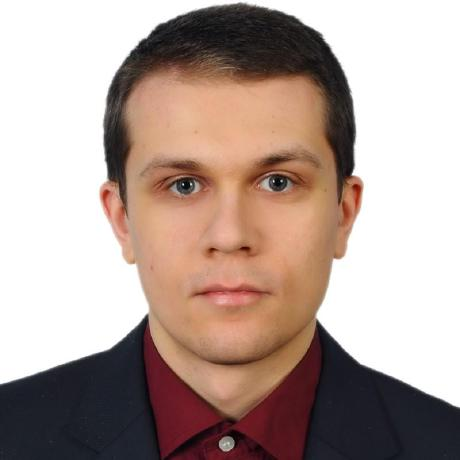
\includegraphics[height=2.7cm]{28454576.jpg}};
\end{tikzpicture}

\begin{rSection}{Work Experience}

    \begin{rSubsection}
        {\bf Cisco Systems Poland Sp. z o.o.}
        {\em Nov. 2023 - Present}
        {\normalfont Software Engineer (grade 008, remote)}{Cracow, PL}

        \item[] {Integrating with the new APIs. Integrating and adapting to the new cloud - FedRAMP. Debugging and resolving production issues. Improving API performance and resolving SLA violations (by introducing cache and rearchitecting). Doing code reviews.}
        \item[] {Technical leader of the \underline{Asset Replacement Enhancements} feature - \url{https://tinyurl.com/rmaasset}}
        \item[] {Stack: Java 17, Maven, Spring Boot, Lombok, Docker, AWS Cloud, JUnit, Mockito, Redis, Splunk, Postman, SonarQube, GitHub Actions, GitHub Copilot, Jira, Confluence.}

    \end{rSubsection}

    \begin{rSubsection}
        {\bf Cisco Systems Poland Sp. z o.o.}
        {\em Jul. 2021 - Oct. 2023}
        {\normalfont Software Engineer (grade 006, remote)}{Cracow, PL}

        \item[] {Maintaining and adding new features and functionalities to Cisco Customer Experience (CX) Cloud solutions.
                    Developing and deploying SaaS software. Shipping cloud-native software in AWS.
                    Creating and maintaining large-scale distributed cloud-native technology stacks that achieve over 99.98\% uptime.}
        \item[] {Stack: Java 11, Maven, Spring Boot, Lombok, Docker, AWS Compute, Kubernetes, K8s, JUnit 5, Mockito 2, Testcontainers, Redis, Aurora, DynamoDB,
                    Elastic Search, KDK, AppDynamics, Rookout, Postman, SonarQube, SonarLint, Git, GitHub, Jira, Confluence, WSL2.}

    \end{rSubsection}

    \begin{rSubsection}
        {\bf Comarch S.A.}
        {\em Jun. 2020 - Nov. 2020}
        {\normalfont Programmer (hybrid)}{Cracow, PL}

        \item[] {Responsible for designing, implementing, and documenting the data archiving process in the loyalty system. Designing and programming
                    automated API tests for handling transactions in the loyalty program. Solution testing.}
        \item[] {Stack: Java 8, Maven, Spring Boot, PostgreSQL, Lombok, Postman, JUnit 4, Git, GitHub, Jira, Confluence.}

    \end{rSubsection}

    \begin{rSubsection}
        {\bf Comarch S.A.}
        {\em Jul. 2019 - Sep. 2019}
        {\normalfont Internship (in person)}{Cracow, PL}

        \item[] {Maintaining and developing a three-layered web application responsible for managing employee vacations.
                    Integrated the system with Rocket Chat server. Implemented REST API for transferring data between the web
                    application and the server. Introduced the Rocket Chat two-factor authentication into the system.
                    Avatar change feature on the UI and image storage in the PostgreSQL.}
        \item[] {Stack: Java 8, Maven, Spring Boot, PostgreSQL, Lombok, Angular, Docker, Git, GitHub, Jira, Confluence.}

    \end{rSubsection}

    \begin{rSubsection}
        {\bf TITUTO sp. z o.o.}
        {\em Feb. 2019 - Apr. 2019}
        {\normalfont Internship (in person)}{Rzeszow, PL}

        \item[] {Responsible for developing mobile applications, testing the TITUTO products and preparing technical documentation.}
        \item[] {Stack: Xamarin, TortoiseSVN.}

    \end{rSubsection}

    \begin{rSubsection}
        {\bf Polskie ePlatnosci S.A.}
        {\em Jul. 2018 - Sep. 2018}
        {\normalfont Junior Specialist of POS picking centre (in person)}
        {Tajecina/Jasionka, PL}

        \item[] {Uploading the software. Configuring and preparing terminals for use in the merchant
                    network. Testing and configuring the hardware. Logistical handling of shipments. Organizational and clerical work.}

    \end{rSubsection}

\end{rSection}

\begin{rSection}{Education}

    {\bf Rzeszow University of Technology, Rzeszow, PL} \hfill {\em Nov. 2022 - Jun. 2023} \\
    Specialization: Project Manager \\
    \url{https://tinyurl.com/przproject}

    {\bf Rzeszow University of Technology, Rzeszow, PL} \hfill {\em Nov. 2021 - Jun. 2022} \\
    Specialization: Master of Business Administration (MBA) \\
    \url{https://tinyurl.com/przmba}

    {\bf Rzeszow University of Technology, Rzeszow, PL} \hfill {\em Feb. 2020 - Jul. 2021} \\
    M. Eng. in Computer Science \\
    Specialization: Technical Computer Science and Telecommunications

    {\bf Fachhochschule Suedwestfalen, Hagen, DE} \hfill {\em Aug. 2019 - Feb. 2020} \\
    Eng. in Computer Science \\
    Specialization: Computer Engineering \\
    \url{https://tinyurl.com/fhswfkocan}

    {\bf Rzeszow University of Technology, Rzeszow, PL} \hfill {\em Sep. 2015 - Feb. 2020} \\
    Eng. in Computer Science \\
    Specialization: Technical Computer Science and Telecommunications \\
    \url{https://tinyurl.com/przkocan}

\end{rSection}

\begin{rSection}{Technical Strengths}

    \begin{itemize}
        \item Programming in object-oriented paradigm.
        \item Knowledge of basic design patterns in Java, RESTful APIs, Clean Code rules, algorithms and data structures.
        \item Hard-working, ambitious, soft skilled.
    \end{itemize}

\end{rSection}

\begin{rSection}{Private Projects}

    \begin{itemize}
        \item \bf Stock Exchange App \normalfont - during my studies, I had the pleasure of being the leader of a team.
              We created a web application, that allowed people to trade shares. We also implemented a special benchmark that simulates stock market transactions.\\
              GitHub: https://github.com/AI-2020-2021-LAB1
        \item \bf Exchange rates and information \normalfont - the Android app displays the current prices of currencies and gold in PLN.
              It also shows the prices of the most popular cryptocurrencies in USD.
              The public Web API of the National Bank of Poland and the public CoinCap API 2.0 were used.
              It also uses the public RSS feed to display the latest news.\\
              Store: https://play.google.com/store/apps/details?id=com.main.app.currency.exchange.rates
    \end{itemize}

\end{rSection}

\begin{rSection}{Interests}

    {Meeting new people, repairing and tuning cars, watching motor sports, cycling, running, playing the stock market, bowling, automating things, IoT}

\end{rSection}

{\footnotesize "I agree to the processing of personal data provided in this document for realising the recruitment process pursuant to the Personal Data
Protection Act of 10 May 2018 (Journal of Laws 2018, item 1000) and in agreement with Regulation (EU) 2016/679 of the European Parliament and of
the Council of 27 April 2016 on the protection of natural persons with regard to the processing of personal data and on the free movement of such
data, and repealing Directive 95/46/EC (General Data Protection Regulation)."}

\end{document}
